%%%%%%%%%%%%%%%%%%%%%%%%%%%%%%%%%%%%%%%%%%%%%%%%%%%%%%%%%%%%%%%%%%%%%%%%%%%%%%%%%%%%
%% --> ScrewDriver te Blackheadborough:
\newcommand{\AUtoKCM}{627.5084}
\newcommand{\AUtoKJM}{2625.5}
%%%%%%%%%%%%%%%%%%%%%%%%%%%%%%%%%%%%%%%%%%%%%%%%%%%%%%%%%%%%%%%%%%%%%%%%%%%%%%%%%%%%
%% \usepackage{fouriernc}
\newcommand{\Func}[1]{{\ensuremath{\mathcal #1}}}
\newcommand{\AGroup}[1]{{\ensuremath{\mathbb #1}}}
%% ------------------------------------------------| ????
\usepackage{epigraph}
\renewcommand{\epigraphwidth}{8.5cm}
%\usepackage{pxfonts}
\usepackage{pifont}
\newcommand{\CycleFirst}{\ding{172}}
\newcommand{\CycleSecond}{\ding{173}}
\newcommand{\CycleThird}{\ding{174}}
\newcommand{\CyclePseudoFirst}{\ding{195}}
\newcommand{\CyclePseudoSecond}{\ding{196}}
%%%%%%%%%%%%%%%%%%%%%%%%%%%%%%%%%%%%%%%%%%%%%%%%%%%%%%%%%%%%%%%%%%%%%%%%%%%%%%%%%%%%
%% Пакет, обеспечивающий адекватную расстановку "русских" кавычек
\usepackage[russian]{quotmark}
%% Теперь для точной расстановки кавычек можно использовать вложенные команды tqt:
%% \tqt{а \tqt{б} в} = ,,а <<б>> в''
%%%%%%%%%%%%%%%%%%%%%%%%%%%%%%%%%%%%%%%%%%%%%%%%%%%%%%%%%%%%%%%%%%%%%%%%%%%%%%%%%%%%
%% Химические пакеты
%\usepackage[compatibility=latest,language=russian]{chemmacros}
\usepackage[version=4]{mhchem}
\usepackage{chemfig}
%\chemsetup{modules=all}
\usepackage{chemnum}
\makeatletter
\def\CF@node@content{\expandafter\expandafter\expandafter
    \printatom\expandafter\expandafter\expandafter
    {\csname atom@\number\CF@cnt@atomnumber\endcsname}%
    \ensuremath{\CF@node@strut}%
}
\makeatother
\renewcommand*\printatom[1]{\ensuremath{\mathsf{#1}}} % from the ChemFig manual
%%%%%%%%%%%%%%%%%%%%%%%%%%%%%%%%%%%%%%%%%%%%%%%%%%%%%%%%%%%%%%%%%%%%%%%%%%%%%%%%%%%%
%% Relied upon \compoundstyle from *chemcompounds*
\usepackage{chemcompounds}
\newcommand{\ConfName}[1]{{\compoundstyle{#1}}}
%
\newcommand{\BB}[1]{{#1}\ConfName{ВВ}}
\newcommand{\BC}[1]{{#1}\ConfName{ВК}}
\newcommand{\CB}[1]{{#1}\ConfName{КВ}}
\newcommand{\CC}[1]{{#1}\ConfName{КК}}
\newcommand{\TT}[1]{{#1}\ConfName{ТТ}}
%%
%%%%%%%%%%%%%%%%%%%%%%%%%%%%%%%%%%%%%%%%%%%%%%%%%%%%%%%%%%%%%%%%%%%%%%%%%%%%%%%%%%%%
%% chemfig setup
\newcommand{\boldbondwidth}{3.5pt}
\setchemfig{angle increment=15}
\setchemfig{arrow offset=12pt}
\setchemfig{atom sep=1.875em}
\setchemfig{bond style={line width=1pt}}
\setchemfig{bond offset=2.5pt}
\setchemfig{bond join=true}
\setchemfig{compound sep=4.5em}
\setchemfig{cram width =\boldbondwidth}
\setchemfig{cram dash width=1pt}
\setchemfig{cram dash sep=2pt}
\setchemfig{cycle radius coeff=0.5}
\setchemfig{double bond sep=3pt}
%%
%%%%%%%%%%%%%%%%%%%%%%%%%%%%%%%%%%%%%%%%%%%%%%%%%%%%%%%%%%%%%%%%%%%%%%%%%%%%%%%%%%%%
% подпись на связях в молекуле, нарисованной в пакете *chemfig*
\newcommand\namebond[4][6.5pt]{\chemmove{\path(#2)--(#3)node[midway,sloped,yshift=#1]{#4};}}

\newcommand\arcbetweennodes[3]{%
  \pgfmathanglebetweenpoints{\pgfpointanchor{#1}{center}}{\pgfpointanchor{#2}{center}}%
  \let#3\pgfmathresult}
%%
\newcommand\arclabel[6][stealth-stealth,shorten <=1pt,shorten >=1pt]{%
  \chemmove{%
    \arcbetweennodes{#4}{#3}\anglestart \arcbetweennodes{#4}{#5}\angleend
    \draw[#1]([shift=(\anglestart:#2)]#4)arc(\anglestart:\angleend:#2);
    \pgfmathparse{(\anglestart+\angleend)/2}\let\anglestart\pgfmathresult
    \node[shift=(\anglestart:#2+1pt)#4,anchor=\anglestart+180,rotate=\anglestart+90,inner sep=0pt, outer sep=0pt]at(#4){#6};}
}
%%
\newcommand{\ChemPicture}[1]{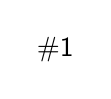
\begin{tikzpicture}\node (ChemFormula) at (0,0){\chemfig{#1}};\end{tikzpicture}}%
%%
%%%%%%%%%%%%%%%%%%%%%%%%%%%%%%%%%%%%%%%%%%%%%%%%%%%%%%%%%%%%%%%%%%%%%%%%%%%%%%%%%%%%%%
%% Немного математических символов
\newcommand{\Energytot}{{\ensuremath E_{tot}}{}}
\newcommand{\EnergyZPE}{{\ensuremath E_{ZPE}}{}}
\newcommand{\EStrain}{{\ensuremath\Func{E}_\varsigma}{}}
\newcommand{\SymGroup}[2]{\ensuremath{\AGroup{#1}_{#2}}}
%%
%%%%%%%%%%%%%%%%%%%%%%%%%%%%%%%%%%%%%%%%%%%%%%%%%%%%%%%%%%%%%%%%%%%%%%%%%%%%%%%%%%%%%%
\usepackage{pgfplotstable}
\pgfplotsset{width=12.5cm,compat=1.15}
%\pgfkeys{/pgf/fpu=true}
\pgfplotstableset{%
  1000 sep={},
  empty cells with = {\ensuremath{-}},
  every head row/.style = {before row=\toprule,after row=\midrule},
  every last row/.style = {after row=\bottomrule},
  %every first column/.style={},
  columns/Tau/.style={int detect,column type=r,column type/.add={}{|},column name={$\tau$}},
  columns/Etot/.style={fixed,fixed zerofill,
    column type=r,
    precision=6,column name=$\Energytot$},
  columns/Emin/.style={fixed,fixed zerofill,precision=6,
    column name={$E_0$},
  },
  columns/Erel/.style={fixed,fixed zerofill,
    column type=r,
    precision=2,%showpos,
    column name={$\Delta\Func{E}$},
    %create on use={create col/expr={2625.5 * {\thisrow{Etot} - \thisrow{Emin}} } },
  }
}